\chapter{Ergebnisse}

Dieses Kapitel stellt die Resultate der verschiedenen Experimente vor und zeigt auf, welche Design-Entscheidungen welche Auswirkungen haben.



\section{Erste Experimente und Debugging}

Der zur Verfügung stehende TensorFlow-Code bietet bereits einige Möglichkeiten, den Trainingsverlauf zu bewerten, da bestimmte Werte während des Trainings als Skalar ausgegeben und in Tensorboard als Verlauf angezeigt werden.
Zu diesen Werten gehören Mittelwerte der Gewichte und Bias-Werte jeder Schicht sowie deren Gradienten und drei Terme aus der Verlustfunktion:

\begin{enumerate}
	\item das \emph{Diskriminator-Loss}: der GAN-Term $ \mathcal{L}_c(D, G) $ der Gesamtverlustfunktion $ R^* $ (s. \autoref{eq:canlosswonoise})
	\item das \emph{Generator-Loss} $ D(\mathbf{x}, G(\mathbf{x})) $: die Bewertung des Diskriminators für den Output des Generators
	\item das \emph{L1-Loss}: der L1-Term $ \lambda \mathcal{L}_{L1}(G) $ der Gesamtverlustfunktion $ R^* $
\end{enumerate}

Ebenso gibt das Netz auch Bilder bzw. Aktivierungen bestimmter Schichten als Bild aus.
Unter diesen Bildausgaben sind neben Input, Target und Output auch die Aktivierungen der letzten Diskriminatorschicht für die Bewertung des realistischen Inputs $ D(\mathbf{x}, \mathbf{y}) $ und für die Bewertung des gefälschten Outputs $ D(\mathbf{x}, G(\mathbf{x})) $.
Diese werden im folgenden mit \emph{Real} und \emph{Fake} respektive bezeichnet.
Das Generator-Loss entspricht hierbei dem Mittelwert aller Aktivierungen von Fake.

Bei einem ersten Trainingslauf wurde das Netz für etwa 200 Epochen trainiert.
Demo-Datasets, die von den Autoren im Paper verwendet und online zur Verfügung gestellt werden, erzielen nach Trainingszeiten in dieser Größenordnung gute Ergebnisse.
In diesem Fall jedoch war der Output immer komplett schwarz, Real komplett weiß und Fake ebenfalls schwarz (s. \autoref{fig:outputsini}).
Letzteres zeigt, dass der Diskriminator maximal in der Lage ist, zwischen gefälschten und realistischen Bildern zu unterscheiden.
Die Verläufe der Losses des ersten Trainingslaufs in \autoref{fig:lossini} zeigen, dass das Diskriminator-Loss sofort auf Null fällt, das Generator-Loss ungewöhnlich große Sprünge aufweist und das L1-Loss nach kürzester Zeit auf einem Plateau stagniert.

% TODO fig:lossini Losses von initial und facades

\begin{figure}
	\centering
	\begin{subfigure}{.19\textwidth}
		\centering
		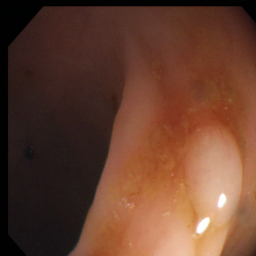
\includegraphics[width=.9\linewidth]{img/results/initial_input}
		\caption{Input}
	\end{subfigure}
	\begin{subfigure}{.19\textwidth}
		\centering
		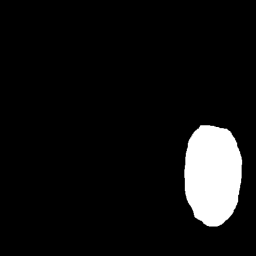
\includegraphics[width=.9\linewidth]{img/results/initial_target}
		\caption{Target}
	\end{subfigure}
	\begin{subfigure}{.19\textwidth}
		\centering
		
\includegraphics[width=.9\linewidth]{img/results/initial_output}
		\caption{Output}
	\end{subfigure}
	\begin{subfigure}{.19\textwidth}
		\centering
		
\includegraphics[width=.9\linewidth,interpolate=false]{img/results/initial_real}
		\caption{Real}
	\end{subfigure}
	\begin{subfigure}{.19\textwidth}
		\centering
		
\includegraphics[width=.9\linewidth,interpolate=false]{img/results/initial_fake}
		\caption{Fake}
	\end{subfigure}
	\caption{Initialer Trainingslauf: ein Datensatz und die dazugehörige Ausgabe des Netzes.}
	\label{fig:outputsini}
\end{figure}

Als Referenz ist in \autoref{fig:lossini} der Trainingsverlauf des Facades-Demo-Datasets aufgezeichnet:
Hier bewegt sich das Diskriminator-Loss auf den Wert 0.5 zu, der Verlauf des Generator-Loss ist sehr viel beständiger und das L1-Loss nimmt stetig ab.

Eine Debugging-Strategie, die \citeauthor{Goodfellow.2016} bei Deep Learning vorschlagen, ist das Trainieren mit einem sehr kleinen Dataset, um zu überprüfen, ob das Netz überhaupt in der Lage ist, aus den Trainingsdaten zu lernen~\cite{Goodfellow.2016}.
Zu diesem Zweck wurde ein Trainingslauf mit drei zufällig gewählten Datensätzen durchgeführt, und schon nach wenigen Trainingsschritten zeigte sich Erfolg (s. \autoref{fig:lossminsamples} und \autoref{fig:outputsminsamples}):

% TODO fig:lossminsamples Losses von min-samples, initial und facades angedeutet

\begin{figure}
	\centering
	\begin{subfigure}{.19\textwidth}
		\centering
		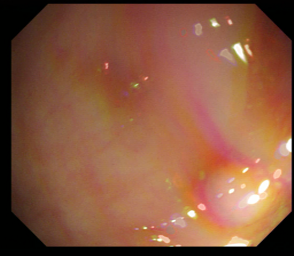
\includegraphics[width=.9\linewidth]{img/results/min_input}
		\caption{Input}
	\end{subfigure}
	\begin{subfigure}{.19\textwidth}
		\centering
		
\includegraphics[width=.9\linewidth]{img/results/min_target}
		\caption{Target}
	\end{subfigure}
	\begin{subfigure}{.19\textwidth}
		\centering
		
\includegraphics[width=.9\linewidth]{img/results/min_output}
		\caption{Output}
	\end{subfigure}
	\begin{subfigure}{.19\textwidth}
		\centering
		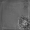
\includegraphics[width=.9\linewidth,interpolate=false]{img/results/min_real}
		\caption{Real}
	\end{subfigure}
	\begin{subfigure}{.19\textwidth}
		\centering
		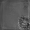
\includegraphics[width=.9\linewidth,interpolate=false]{img/results/min_fake}
		\caption{Fake}
	\end{subfigure}
	\caption{Durchlauf mit minimaler Anzahl Samples: Datensatz mit Ausgabe}
	\label{fig:outputsminsamples}
\end{figure}

Der Output ist nicht mehr leer, sondern nahe am Target, und Real und Fake sind sehr ähnlich.
Außerdem ist das Diskriminator-Loss nicht mehr auf Null, das Generator-Loss tendiert zu niedrigeren Werten und das L1-Loss verläuft monoton fallend.
Ein weiterer Trainingslauf mit den vollen Trainingsdaten und doppelter Trainingsdauer war dann erfolgreicher und führte zu ähnlich guten Ergebnissen wie der zweite Durchlauf mit minimaler Anzahl an Samples.



\section{Metriken}

Die \gls{giana} Challenge gibt zwei Metriken vor, um die Qualität der produzierten Segmentierungen zu bewerten: den Jaccard-Index~\cite{Jaccard.1901} und den Sørensen–Dice-Koeffizient~\cite{Srensen.1948,Dice.1945}.
Der Jaccard-Index ist auch bekannt als \gls{iou}, also Schnittmenge geteilt durch Vereinigungsmenge.
Die beiden Mengen sind in diesem Fall die Flächen mit Polypenpixeln im Target und im Output; die Schnittmenge ist die Überlappung beider Flächen.
Der \gls{iou} berechnet sich anhand der Anzahl wahr positiver (TP), falsch positiver (FP) und falsch negativer (FN) Samples bzw. anhand der Mengen A und B folgendermaßen:

\begin{equation}
J(A, B) = \frac{| A \cap B |}{| A \cup B |} = \frac{TP}{TP + FP + FN}
\end{equation}

Der Sørensen–Dice-Koeffizient ist identisch mit dem F1-Score, der das harmonische Mittel von Genauigkeit und Trefferquote ist.
Er ist folgendermaßen definiert:

\begin{equation}
SD(A, B) = \frac{2 \ | A \cap B |}{| A | + | B |} = \frac{2 \ TP}{2 \ TP + FP + FN}
\end{equation}

Die Werte beider Metriken liegen zwischen 0 und 1.
Im Gegensatz zum \gls{iou} erfüllt der F1-Score die Dreiecksungleichung nicht, wodurch nur der \gls{iou} sich als Distanzmaß eignet.
Beide Metriken sind insofern gleichwertig als dass sich der Wert einer Metrik durch den Wert der anderen berechnen lässt:

\begin{equation}
J = \frac{SD}{2 - SD} \ , \quad SD = \frac{2 \ J}{1 + J}
\end{equation}

Es ist direkt ersichtlich, dass der \gls{iou} nicht korrekt klassifizierte Pixel, also solche außerhalb der Schnittmenge, stärker bestraft als der F1-Score.
In den nachfolgenden Experimenten wird der Einfachheit wegen nur der \gls{iou} angegeben, da dieser der pessimistischere der beiden Werte ist und der F1-Score sich ohne Umschweife aus dem Wert \gls{iou} berechnen lässt.



\section{Batch-Größen}\label{sec:batchsize}

Da die ersten Trainingsläufe mit den Standardparametern des Netzes durchgeführt wurden, betrug die Batch-Größe immer 1.
Das \gls{can} braucht bei einer solchen Batch-Größe sehr lange, bis der Generator überhaupt anfängt etwas zu lernen.
Möglicherweise liegt die Ursache dafür in der Tatsache, dass das Netz \emph{zu wenig Varianz pro Batch} und damit pro Lernschritt zu sehen bekommt und es deshalb lange dauert, bis der Generator etwas lernt.

Zur Überprüfung dieser Hypothese wurden verschiedene Batch-Größen evaluiert.
Oftmals werden in solchen Fällen Zweierpotenzen gewählt, deshalb wurden hier die Batch-Größen 1, 2, 4, 8, 16, 32 und 64 getestet.
Für jede Batch-Größe wurden zwei Trainingsläufe durchgeführt, um mögliche Varianzen beim Training zu einem gewissen Grad einschätzen zu können.
Die Dauer jedes Trainingslaufs betrug 600 Epochen, was bei unterschiedlichen Batch-Größen zu einer unterschiedlichen Anzahl von Trainingsschritten führt.

In \autoref{fig:lossb0124} wird ersichtlich, dass das Netz erst bei einer Batch-Größe über 2 in der Lage ist, von Anfang an zu lernen.
Es zeigt sich ebenso, dass folgende Muster in den Verläufen aller Batch-Größen sehr zuverlässig korrelieren:

\begin{itemize}
	\item Diskriminator-Loss: Fallen oder Zurückfallen auf Null 
	\item Generator-Loss: steil ansteigende Werte mit sägezahnartigen Verläufen
	\item L1-Loss: Stagnieren auf einem Niveau, dessen Wert bei allen Trainingsläufen ähnlich ausfällt
	\item \gls{iou}: Stagnieren bei Null oder Verschlechterung
	\item Diskriminator und Generator in jeweils allen Schichten: Stagnieren von Gewichten und Bias-Werten und Zurückfallen auf Null der Gradienten
\end{itemize}

All diese Verläufe und besonders das letzte Muster sprechen dafür, dass der Generator in solchen Phasen nicht in der Lage ist, irgendetwas zu lernen, das er dem Diskriminator entgegen setzen kann.

% TODO fig:lossb0124 alle 4 Losses (loss|mean_iou_val) von 2017/b0[124]/ step_relative(?)
% TODO erklären relativ skaliert gesamter Trainingsverlauf auf maximale Breite
% TODO erklären IoU nur auf val

Um herauszufinden, welche Batch-Größe minimal notwendig ist, damit das Netz von Beginn an lernen kann, wurden auch zwei Trainingsläufe mit Batch-Größe 3 durchgeführt.
\autoref{fig:loss3} zeigt, dass alle Durchläufe mit dieser Batch-Größe in Bezug auf den \gls{iou} kontinuierlich ansteigen und eine Art Schranke erreichen, ab der die Ergebnisse nicht mehr besser werden.
Auf diesem Niveau sind die auf den Trainingsdaten erzeugten Outputs visuell akzeptabel, aber der Diskriminator ist dennoch in der Lage, die gefälschten Exemplare sicher zu identifizieren (s. \autoref{fig:outputsb03}).

% TODO fig:lossb03 Losses 2017/b03/ step_step (Hinweis?)

\begin{figure}
	\centering
	\begin{subfigure}{.19\textwidth}
		\centering
		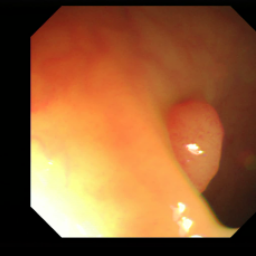
\includegraphics[width=.9\linewidth]{img/results/b03_input}
		\caption{Input}
	\end{subfigure}
	\begin{subfigure}{.19\textwidth}
		\centering
		
\includegraphics[width=.9\linewidth]{img/results/b03_target}
		\caption{Target}
	\end{subfigure}
	\begin{subfigure}{.19\textwidth}
		\centering
		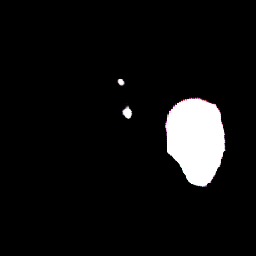
\includegraphics[width=.9\linewidth]{img/results/b03_output}
		\caption{Output}
	\end{subfigure}
	\begin{subfigure}{.19\textwidth}
		\centering
		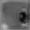
\includegraphics[width=.9\linewidth,interpolate=false]{img/results/b03_real}
		\caption{Real}
	\end{subfigure}
	\begin{subfigure}{.19\textwidth}
		\centering
		
\includegraphics[width=.9\linewidth,interpolate=false]{img/results/b03_fake}
		\caption{Fake}
	\end{subfigure}
	\caption{Durchlauf mit Batch-Größe 3 nach 6900 Schritten (ca. 78 Epochen): Datensatz mit Ausgabe}
	\label{fig:outputsb03}
\end{figure}

Man könnte vermuten, dass das Netz in einem lokalen Minimum angelangt ist, und hoffen, dass bei anderen Batch-Größen über 3 sich ähnlich konsistente Ergebnisse zeigen, bei denen die Schranke sich kontinuierlich nach oben verschiebt.
Tatsächlich aber ergibt sich eine solche Konsistenz erst wieder bei einer Batch-Größe von 64.
Zusätzlich wurde die logarithmische Mitte zwischen 32 und 64, also $ round(2^{5,5}) = 45 $ evaluiert; auch hier waren beide Trainingsläufe ähnlich und fielen in keines der oben genannten Muster von Zurückfallen und Stagnation.
Insgesamt sind die Trainingsverläufe sehr glatt (s. \autoref{fig:lossb4564}) und \autoref{fig:outputsb64} zeigt, dass der Diskriminator kaum noch in der Lage ist zwischen realistisch und gefälscht zu unterscheiden.

% TODO fig:lossb4564 Losses 2017/b(45|64) step_step(?)

\begin{figure}
	\centering
	\begin{subfigure}{.19\textwidth}
		\centering
		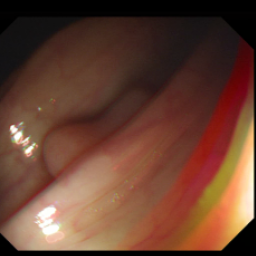
\includegraphics[width=.9\linewidth]{img/results/b64_input}
		\caption{Input}
	\end{subfigure}
	\begin{subfigure}{.19\textwidth}
		\centering
		
\includegraphics[width=.9\linewidth]{img/results/b64_target}
		\caption{Target}
	\end{subfigure}
	\begin{subfigure}{.19\textwidth}
		\centering
		
\includegraphics[width=.9\linewidth]{img/results/b64_output}
		\caption{Output}
	\end{subfigure}
	\begin{subfigure}{.19\textwidth}
		\centering
		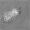
\includegraphics[width=.9\linewidth,interpolate=false]{img/results/b64_real}
		\caption{Real}
	\end{subfigure}
	\begin{subfigure}{.19\textwidth}
		\centering
		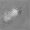
\includegraphics[width=.9\linewidth,interpolate=false]{img/results/b64_fake}
		\caption{Fake}
	\end{subfigure}
	\caption{Durchlauf mit Batch-Größe 64 am Ende des Trainings (600 Epochen): Datensatz mit Ausgabe}
	\label{fig:outputsb64}
\end{figure}

Eine sehr hohe Batch-Größe wie 45 oder 64 zu wählen wäre demnach sinnvoll, um gute und vor allem konsistente Ergebnisse zu bekommen.
Allerdings sind solch hohe Batch-Größen aufgrund von begrenztem Arbeitsspeicher nicht erstrebenswert.
Stattdessen wurde versucht, einen guten Kompromiss in Form einer geringeren Batch-Größe auszuwählen.

In \autoref{fig:lossworst} und \autoref{fig:lossbest} sind jeweils der schlechtere und der bessere Durchlauf jeder Batch-Größe zwischen 3 und 32 abgebildet.
Es lässt sich zwar kein klarer Trend ausmachen, welche Batch-Größe zu mehr Stabilität und gleichzeitig besseren Ergebnissen tendiert.
Allerdings lässt sich beobachten, dass bei den besseren Trainingsläufen Batch-Größe 4 zu einem ähnlichen IoU-Plateau wie Batch-Größe 3 tendiert.
Außerdem tritt selbst bei dem besseren Trainingslauf von Batch-Größe 8 eine lange Periode von katastrophalem Rückfall auf.

% TODO fig:lossworst b03/A b04/A b08/B b16/B b32/B

% TODO fig:lossbest b03/B b04/B b08/A b16/A b32/A

Hätte man allerdings bei dieser Batch-Größe und dem besseren Durchlauf das Training an dem Punkt beendet, auf dem der \gls{iou} am höchsten war, wäre dieser Wert weniger als 2 Prozentpunkte unter dem Schlusswert des besseren Durchlaufs von Batch-Größe 32 gewesen.
\emph{Early Stopping} ist eine Methode zur Vermeidung von Overfitting, die das Training nach einem Stoppkriterium beendet.
Dieses Kriterium ist dann erfüllt, wenn der Fehler auf den Trainingsdaten kleiner wird, gleichzeitig aber der Fehler auf den Validierungsdaten anfängt zu steigen und nach einer gewissen Geduldsperiode nicht wieder gesunken ist~\cite{Goodfellow.2016}.

\autoref{fig:loss081632} zeigt alle Trainingsläufe der Batch-Größen 8, 16 und 32.
Wenn wir jeden dieser Verläufe so betrachten, als wäre er mit Early Stopping bei einer Geduldsperiode von bspw. 1000 Trainingsschritten durchgeführt worden, erhalten wir zwei Early-Stopping-Werte pro Batch-Größe.
Die besten und schlechtesten ES-Werte sind in \autoref{fig:es081632} visualisiert und zeigen, dass Batch-Größe 8 zwar die geringste Varianz bietet, während Batch-Größe 32 einen höheren maximalen ES-Wert bietet bei ähnlich geringer Varianz.
Außerdem ist bei Batch-Größe 32 möglicherweise noch nicht der höchstmögliche beste ES-Wert erreicht, da im besseren Trainingsverlauf noch keine Verschlechterung des \gls{iou} stattgefunden hat.
Aus diesem Grund wurde 32 als die Batch-Größe aller folgenden Experimente gewählt.

% TODO fig:loss081632 Losses 8, 16, 32

% TODO fig:es081632 Early Stopping Werte min und max als 2 Linien von b081632



\section{Dataset Augmentation}



\section{Deaktivieren von Dropout zur Testzeit}

Um den Effekt der Deaktivierung von Dropout zur Testzeit zu untersuchen, wurde folgendes Evaluierungsszenario erstellt:
Der \gls{iou} wurde einmal auf dem gesamten Test-Sub-Dataset CVC-612 und einmal auf einem einzelnen, zufällig ausgewählten Bild berechnet.
Hierbei wurde einmal Dropout zur Testzeit aktiviert und einmal deaktiviert.
Für jede dieser vier Varianten wurden 10 Testläufe durchgeführt.

Für CVC-612 ergab sich bei aktivem Dropout ein mittlerer \gls{iou} von 0,2073 mit einer Standardabweichung von 0,012, bei deaktiviertem Dropout hingegen ein konstanter Wert von 0,2117.
Dies bedeutet nicht nur eine Verbesserung des Durchschnittswertes um 0,44 Prozentpunkte, sondern auch eine Eliminierung der Varianz in den Ergebnissen.

Die Berechnung auf dem einzelnen Bild ergab bei aktivem Dropout einen mittleren \gls{iou} von 0,4243 mit Standardabweichung 0,0412, bei deaktiviertem Dropout ergab sich ein konstanter Wert von 0,4365.
Dies entspricht einer Verbesserung vom durchschnittlichen zum konstanten Wert von sogar 1,22 Prozentpunkten.

Entsprechend diesen Ergebnissen wurde Dropout zur Testzeit standardmäßig deaktiviert.



\section{Umkehren der Lernrichtung}

\citeauthor{Isola.2017} explorieren das Training verschiedenster Input-Target-Paare, sei es Labels zu Straßenszene, Vogelperspektive zu Kartenansicht oder Tag zu Nacht.
Sie experimentieren auch mit einer Umkehrung der Lernrichtung, also dass z.~B. Nacht zu Tag, Kartenansicht zu Vogelperspektive oder Straßenszene zu Labels gelernt wird.

Interessehalber wurde das \gls{can} im Rahmen dieser Arbeit auch für ein paar Epochen mit umgekehrter Lernrichtung trainiert; die Binärmaske war also der Input und die Originalszene das Target.
Die Ergebnisse in \autoref{fig:lossbtoa} und \autoref{fig:outputsbtoa} zeigen, wie schnell das Netz in diesem Fall selbst mit einer Batch-Größe von 1 lernt.
Die visuelle Qualität der Ergebnisse ist für die kurze Trainingsdauer gut, und das Training verläuft ähnlich stabil wie das eines Demo-Datasets der \glspl{can}.

% TODO fig:lossbtoa Losses BtoA

\begin{figure}
	\centering
	\begin{subfigure}{.19\textwidth}
		\centering
		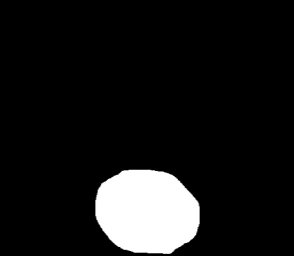
\includegraphics[width=.9\linewidth]{img/results/btoa_input}
		\caption{Input}
	\end{subfigure}
	\begin{subfigure}{.19\textwidth}
		\centering
		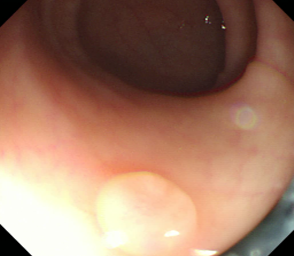
\includegraphics[width=.9\linewidth]{img/results/btoa_target}
		\caption{Target}
	\end{subfigure}
	\begin{subfigure}{.19\textwidth}
		\centering
		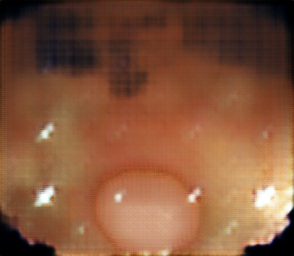
\includegraphics[width=.9\linewidth]{img/results/btoa_output}
		\caption{Output}
	\end{subfigure}
	\begin{subfigure}{.19\textwidth}
		\centering
		
\includegraphics[width=.9\linewidth,interpolate=false]{img/results/btoa_real}
		\caption{Real}
	\end{subfigure}
	\begin{subfigure}{.19\textwidth}
		\centering
		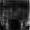
\includegraphics[width=.9\linewidth,interpolate=false]{img/results/btoa_fake}
		\caption{Fake}
	\end{subfigure}
	\caption{Durchlauf mit umgekehrter Lernrichtung am Ende des Trainings (ca. 18 Epochen): Datensatz mit Ausgabe}
	\label{fig:outputsbtoa}
\end{figure}

Dies lässt den Schluss zu, dass \glspl{can} zwar grundsätzlich darauf ausgelegt sind, eine Repräsentation einer Szene in eine andere zu konvertieren, aber die Ziel-Repräsentation sollte visuell komplex sein.
Falls die Ziel-Repräsentation zu spärlich ist, wie im Fall von diskreten Labels einer Straßenszene oder dem Binärbild einer Polypensegmentierung, dann bekommt der Generator offensichtlich nicht genug Lernmaterial, um von Anfang an erfolgreich zu lernen.
Die Erhöhung der Batch-Größe wie oben beschrieben ist demnach ein sinnvolles Mittel, um die \glspl{can} für spärliche Outputs nutzbarer zu machen.



\section{L1-Loss ohne GAN-Term}

Bei der Generierung von diskreten Labels aus einer Straßenszene untersuchen \citeauthor{Isola.2017}, wie gut sich die verschiedenen Bestandteile der Verlustfunktion für diese Aufgabe eignen.
Sowohl hinsichtlich der Pro-Pixel-Genauigkeit als auch bei der Pro-Klassen-Genauigkeit und dem Multiklassen-IoU schneidet das L1-Loss alleine deutlich besser ab als der GAN-Term alleine.
(Nutzt man nur das L1-Loss, ist das Netz letztendlich nur ein \gls{dcgan} in U-Net-Struktur.)
Letzteres erreicht Werte, die zwischen 12 und 14 Prozentpunkte schlechter als die des L1-Loss alleine sind.

Nimmt man hingegen die Kombination aus L1-Loss und GAN-Term, welche das \gls{can} von einem reinen L1-getriebenen oder einem bloßen \gls{dcgan} unterscheidet, sind die Ergebnisse ebenfalls etwas schlechter als wenn man nur das L1-Loss für solche Daten nutzt.
Allerdings unterliegt hier das \gls{can} nur mit 3 bis 6 Prozentpunkten.

Auch in dieser Arbeit wurde untersucht, ob das reine L1-Loss bessere Ergebnisse erzielt als die Kombination aus L1-Loss und GAN-Term.
Dazu wurden je drei Testläufe à 250 Epochen durchgeführt für das Baseline-Modell mit kombinierten Losses und das Modell mit nur L1-Loss.
Die Verläufe in \autoref{fig:lossbaselinel1} zeigen, dass das reine L1-basierte Netz am Ende des Trainings sowohl im Durchschnitt als auch beim besten und schlechtesten Wert besser abschneidet als das CAN-Modell.
Der Durchschnittswert des \gls{can} liegt 4,29 Prozentpunkte unter dem des L1-getriebenen Netzes, während immerhin die Standardabweichung der Schlusswerte um 0,42 Prozentpunkte geringer ist.

% TODO fig:lossbaselinel1 Losses 2018_b32/(baseline|only_L1) bis step 2000

Somit ist nicht nur bei einer Multiklassen-Segmentierung, sondern auch bei einer binären Segmentierung das reine L1-Loss knapp besser als die kombinierte Verlustfunktion.
